\chapter{Состояние вопроса. Цель и задачи исследования} \label{chapt1}

\section{Обзор влияния изнашивания режущей кромки дискового режущего инструмента на силу сопротивления резанию} \label{sect1_1}

\def\slantfrac#1#2{ \hspace{3pt}\!^{#1}\!\!\hspace{1pt}/
	\hspace{2pt}\!\!_{#2}\!\hspace{3pt}
} %Макрос для красивых дробей в строчку (например, 1/2)

%Мы можем сделать \textbf{жирный текст} и \textit{курсив}.
На силовые показатели процесса разрушения \todo{прочных снежно ледяных образований (ПСЛО)} дисковым режущим инструментом, кроме геометрических параметров \todo{[Ганжа]}, скорости резания \todo{[Ковалевич]} и температурных режимов \todo{[Каптюк]}, также влияет и степень износа режущей кромки инструмента. В \todo{[Барон]} предлагается использовать классификацию по типу износа:
\begin{enumerate}
	\item с сохранением формоустойчивости (изменение только радиуса закругления режущей кромки);
	\item с потерей формоустойчивости (изменение радиуса закругления и деформация (изгиб) режущей кромки).
\end{enumerate}
Второй класс износа характеризуется либо нарушением технических требований изготовления резца (термообработка), либо авариными режимами работы (заклинивание). Поэтому вторым классом характера износа можно пренебречь. Отсюда следует что износ дискового режущего инструмента характеризуется радиусом закругления $R$ режущей кромки. Так при увеличении радиуса закругления рабочей кромки  с 1,5 до 4,5 мм, т.е. в 3 раза, сила сопротивления резанию увеличивалась в среднем в 2 раза. Такое увеличение наблюдалось на песчаниках выше средней крепости ($p_{k} = 100\div110\ \slantfrac{\text{кГ}}{\text{мм}^{2}}$)
Лед ($12\div76\ \slantfrac{\text{кГ}}{\text{мм}^{2}}$)

Также следует отметить эффект самозатачивания режущей кромки дискового инструмента. Эффект наблюдается только для резцов из однородного материала и не зависит от свойств разрушаемой породы. Радиус самозатачивания в среднем равен 1,3 мм.
\section{Анализ методов контроля}
\section{Анализ методов контроля силы сопротивления резанию рабочих органов строительно-дорожных и уборочных машин при взаимодействии с разрушаемой средой}
Наиболее распространённым методом контроля силовых параметров рабочих органов строительно-дорожных и уборочных машин при взаимодействии с разрушаемой средой является динамометрический метод. Он заключается в измерении деформации, вызываемою прикладываемым усилием, в упругом элементе. Существует несколько способов измерения деформации: механический, гидравлический, электрический.
\begin{figure}[ht] 
	\center
	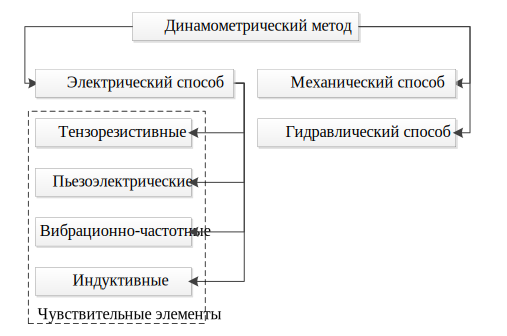
\includegraphics{MetodsControl}
	\caption{Методы контроля силовых параметров} 
	\label{img:MetodsControl}  
\end{figure}

Самым простым является механический способ так как представляет из себя прибор со шкалой либо автоматический самописец. Однако применение этого способа не целесообразно, так как имеются многочисленные недостатки, такие как: громоздкость чувствительного элемента, необходимость постоянной поверки и тарировки, не высокая точность из-за механического способа передачи информации, сложность считывания информации и т.д.

Гидравлический способ имеет в основном узко специализированное применение и не подходит для контроля силовых параметров рабочих органов из-за дороговизны и сложности конструкции.

Самым подходящим способом контроля является электрический. Он обеспечивает преобразование деформаций в электрический сигнал, который легко обрабатывать записывать и хранить. Так же одним из важнейших достоинств метода является малый размер чувствительных элементов, позволяющий устанавливать их в труднодоступных местах.

Электрический способ контроля силовых параметров обычно классифицирую в зависимости от используемых чувствительных элементов см. рисунок~\ref{img:MetodsControl}. Наиболее распространёнными являются тензорезистивные чувствительные элементы, так как:
\begin{itemize}
	\item обеспечивают достаточно высокую точность преобразования деформаций в электрический сигнал;
	\item наилучшим образом удовлетворяют критерию стоимость эффективность;
	\item могут использоваться при действии статических и динамических нагрузок;
	\item имеют линейную характеристику выходного сигнала \todo{[91]}.
\end{itemize}

\begin{table} [htbp]
	\centering
	\captionsetup{width=15cm}
	\caption{Название таблицы}\label{Ts0Sib}%
	\begin{tabular}{| p{3cm} | p{3cm} | p{3cm} | p{4cm}l |}
		\hline
		Месяц   & \centering $T_{min}$, К & \centering $T_{max}$, К &\centering  $(T_{max} - T_{min})$, К & \\
		\hline
		\hline
		Декабрь &\centering  253.575   &\centering  257.778    &\centering      4.203  &   \\
		Январь  &\centering  262.431   &\centering  263.214    &\centering      0.783  &   \\
		Февраль &\centering  261.184   &\centering  260.381    &\centering     $-$0.803  &   \\
		\hline
	\end{tabular}
\end{table}


\section{Ссылки} \label{sect1_2}
Сошлёмся на библиографию. Одна ссылка: \cite[с.~54]{Sokolov}\cite[с.~36]{Gaidaenko}. Две ссылки: \cite{Sokolov,Gaidaenko}. Много ссылок:  \cite[с.~54]{Lermontov,Management,Borozda} \cite{Lermontov,Management,Borozda,Marketing,Constitution,FamilyCode,Gost.7.0.53,Razumovski,Lagkueva,Pokrovski,Sirotko,Lukina,Methodology,Encyclopedia,Nasirova,Berestova,Kriger}. И ещё немного ссылок: \cite{Article,Book,Booklet,Conference,Inbook,Incollection,Manual,Mastersthesis,Misc,Phdthesis,Proceedings,Techreport,Unpublished}. \cite{medvedev2006jelektronnye, CEAT:CEAT581, doi:10.1080/01932691.2010.513279,Gosele1999161,Li2007StressAnalysis, Shoji199895,test:eisner-sample,AB_patent_Pomerantz_1968,iofis_patent1960}

%Попытка реализовать несколько ссылок на конкретные страницы для стандартной реализации:[\citenum{Sokolov}, с.~54; \citenum{Gaidaenko}, с.~36].

%Несколько источников мультицитата \cites[vii--x, 5, 7]{Sokolov}[v--x, 25, 526]{Gaidaenko} поехали дальше

Ссылки на собственные работы:~\cite{vakbib1, confbib1}

Сошлёмся на приложения: Приложение \ref{AppendixA}, Приложение \ref{AppendixB2}.

Сошлёмся на формулу: формула \eqref{eq:equation1}.

Сошлёмся на изображение: рисунок \ref{img:knuth}.

%\newpage
%============================================================================================================================

\section{Формулы} \label{sect1_3}

Благодаря пакету \textit{icomma}, \LaTeX~одинаково хорошо воспринимает в качестве десятичного разделителя и запятую ($3,1415$), и точку ($3.1415$).

\subsection{Ненумерованные одиночные формулы} \label{subsect1_3_1}

Вот так может выглядеть формула, которую необходимо вставить в строку по тексту: $x \approx \sin x$ при $x \to 0$.

А вот так выглядит ненумерованая отдельностоящая формула c подстрочными и надстрочными индексами:
\[
(x_1+x_2)^2 = x_1^2 + 2 x_1 x_2 + x_2^2
\]

При использовании дробей формулы могут получаться очень высокие:
\[
  \frac{1}{\sqrt{2}+
  \displaystyle\frac{1}{\sqrt{2}+
  \displaystyle\frac{1}{\sqrt{2}+\cdots}}}
\]

В формулах можно использовать греческие буквы:
\[
\alpha\beta\gamma\delta\epsilon\varepsilon\zeta\eta\theta\vartheta\iota\kappa\lambda\\mu\nu\xi\pi\varpi\rho\varrho\sigma\varsigma\tau\upsilon\phi\varphi\chi\psi\omega\Gamma\Delta\Theta\Lambda\Xi\Pi\Sigma\Upsilon\Phi\Psi\Omega
\]


Для красивых дробей (например, в индексах) можно добавить макрос
\verb+\slantfrac+ и писать $\slantfrac{1}{2}$ вместо $1/2$.
%\newpage
%============================================================================================================================

\subsection{Ненумерованные многострочные формулы} \label{subsect1_3_2}

Вот так можно написать две формулы, не нумеруя их, чтобы знаки равно были строго друг под другом:
\begin{align}
  f_W & =  \min \left( 1, \max \left( 0, \frac{W_{soil} / W_{max}}{W_{crit}} \right)  \right), \nonumber \\
  f_T & =  \min \left( 1, \max \left( 0, \frac{T_s / T_{melt}}{T_{crit}} \right)  \right), \nonumber
\end{align}

Выровнять систему ещё и по переменной $ x $ можно, используя окружение \verb|alignedat| из пакета \verb|amsmath|. Вот так: 
\[
    |x| = \left\{
    \begin{alignedat}{2}
        &&x, \quad &\text{eсли } x\geqslant 0 \\
        &-&x, \quad & \text{eсли } x<0
    \end{alignedat}
    \right.
\]
Здесь первый амперсанд (в исходном \LaTeX описании формулы) означает выравнивание по~левому краю, второй "--- по~$ x $, а~третий "--- по~слову <<если>>. Команда \verb|\quad| делает большой горизонтальный пробел.

Ещё вариант:
\[
    |x|=
    \begin{cases}
    \phantom{-}x, \text{если } x \geqslant 0 \\
    -x, \text{если } x<0
    \end{cases}
\]

Кроме того, для  нумерованых формул \verb|alignedat|  делает вертикальное
выравнивание номера формулы по центру формулы. Например,  выравнивание компонент вектора:
\begin{equation}
 \label{eq:2p3}
 \begin{alignedat}{2}
{\mathbf{N}}_{o1n}^{(j)} = \,{\sin} \phi\,n\!\left(n+1\right)
         {\sin}\theta\,
         \pi_n\!\left({\cos} \theta\right)
         \frac{
               z_n^{(j)}\!\left( \rho \right)
              }{\rho}\,
           &{\boldsymbol{\hat{\mathrm e}}}_{r}\,+   \\
+\,
{\sin} \phi\,
         \tau_n\!\left({\cos} \theta\right)
         \frac{
            \left[\rho z_n^{(j)}\!\left( \rho \right)\right]^{\prime}
              }{\rho}\,
            &{\boldsymbol{\hat{\mathrm e}}}_{\theta}\,+   \\
+\,
{\cos} \phi\,
         \pi_n\!\left({\cos} \theta\right)
         \frac{
            \left[\rho z_n^{(j)}\!\left( \rho \right)\right]^{\prime}
              }{\rho}\,
            &{\boldsymbol{\hat{\mathrm e}}}_{\phi}\:.
\end{alignedat}
\end{equation}

Ещё об отступах. Иногда для лучшей <<читаемости>> формул полезно
немного исправить стандартные интервалы \LaTeX с учётом логической
структуры самой формулы. Например в формуле~\ref{eq:2p3} добавлен
небольшой отступ \verb+\,+ между основными сомножителями, ниже
результат применения всех вариантов отступа:
\begin{align*}
\backslash! &\quad f(x) = x^2\! +3x\! +2 \\
  \mbox{по-умолчанию} &\quad f(x) = x^2+3x+2 \\
\backslash, &\quad f(x) = x^2\, +3x\, +2 \\
\backslash{:} &\quad f(x) = x^2\: +3x\: +2 \\
\backslash; &\quad f(x) = x^2\; +3x\; +2 \\
\backslash \mbox{space} &\quad f(x) = x^2\ +3x\ +2 \\
\backslash \mbox{quad} &\quad f(x) = x^2\quad +3x\quad +2 \\
\backslash \mbox{qquad} &\quad f(x) = x^2\qquad +3x\qquad +2
\end{align*}


Можно использовать разные математические алфавиты:
\begin{align}
\mathcal{ABCDEFGHIJKLMNOPQRSTUVWXYZ} \nonumber \\
\mathfrak{ABCDEFGHIJKLMNOPQRSTUVWXYZ} \nonumber \\
\mathbb{ABCDEFGHIJKLMNOPQRSTUVWXYZ} \nonumber
\end{align}

Посмотрим на систему уравнений на примере аттрактора Лоренца:

\[ 
\left\{
  \begin{array}{rl}
    \dot x = & \sigma (y-x) \\
    \dot y = & x (r - z) - y \\
    \dot z = & xy - bz
  \end{array}
\right.
\]

А для вёрстки матриц удобно использовать многоточия:
\[ 
\left(
  \begin{array}{ccc}
  	a_{11} & \ldots & a_{1n} \\
  	\vdots & \ddots & \vdots \\
  	a_{n1} & \ldots & a_{nn} \\
  \end{array}
\right)
\]


%\newpage
%============================================================================================================================
\subsection{Нумерованные формулы} \label{subsect1_3_3}

А вот так пишется нумерованая формула:
\begin{equation}
  \label{eq:equation1}
  e = \lim_{n \to \infty} \left( 1+\frac{1}{n} \right) ^n
\end{equation}

Нумерованых формул может быть несколько:
\begin{equation}
  \label{eq:equation2}
  \lim_{n \to \infty} \sum_{k=1}^n \frac{1}{k^2} = \frac{\pi^2}{6}
\end{equation}

Впоследствии на формулы (\ref{eq:equation1}) и (\ref{eq:equation2}) можно ссылаться.

Сделать так, чтобы номер формулы стоял напротив средней строки, можно, используя окружение \verb|multlined| (пакет \verb|mathtools|) вместо \verb|multline| внутри окружения \verb|equation|. Вот так:
\begin{equation} % \tag{S} % tag - вписывает свой текст 
  \label{eq:equation3}
    \begin{multlined}
        1+ 2+3+4+5+6+7+\dots + \\ 
        + 50+51+52+53+54+55+56+57 + \dots + \\ 
        + 96+97+98+99+100=5050 
    \end{multlined}
\end{equation}

Используя команду \verb|\labelcref| из пакета \verb|cleveref|, можно
красиво ссылаться сразу на несколько формул
(\labelcref{eq:equation1,eq:equation3,eq:equation2}), даже перепутав
порядок ссылок \verb|(\labelcref{eq:equation1,eq:equation3,eq:equation2})|.

